\documentclass[12pt, a4paper]{article}

\usepackage{amsmath}
\usepackage{amsfonts}
\usepackage{graphicx}
\usepackage{pdfpages}
\usepackage[titletoc, title]{appendix}
\usepackage{hyperref}
\hypersetup{
    colorlinks=true,
    linkcolor=blue,
    filecolor=magenta,      
    urlcolor=cyan,
}


\def\vb{\boldsymbol{b}}
\def\vh{\boldsymbol{h}}
\def\vw{\boldsymbol{w}}
\def\vx{\boldsymbol{x}}
\def\vy{\boldsymbol{y}}
\def\vz{\boldsymbol{z}}
\def\v1{\boldsymbol{1}}

\def\vI{\boldsymbol{I}}
\def\vW{\boldsymbol{W}}
\def\vX{\boldsymbol{X}}
\def\vY{\boldsymbol{Y}}

\def\vtheta{\boldsymbol{\theta}}
\def\vmu{\boldsymbol{\mu}}
\def\vbeta{\boldsymbol{\beta}}
\def\vSigma{\boldsymbol{\Sigma}}

\def\rmx{\mathrm{x}}

\def\vrmx{\boldsymbol{\mathrm{x}}}
\def\vrmy{\boldsymbol{\mathrm{y}}}

\def\bbE{\mathbb{E}}
\def\bbX{\mathbb{X}}

\DeclareMathOperator*{\relu}{ReLU}
\DeclareMathOperator*{\argmax}{arg\,max}
\DeclareMathOperator*{\argmin}{arg\,min}
\DeclareMathOperator*{\softmax}{softmax}

\newcommand{\egvx}[1]{\boldsymbol{x}^{(#1)}}
\newcommand{\egvy}[1]{\boldsymbol{y}^{(#1)}}
\newcommand{\egx}[1]{x^{(#1)}}
\newcommand{\egy}[1]{y^{(#1)}}
\newcommand{\eghy}[1]{\hat{y}^{(#1)}}

\newcommand{\expect}[3]{\mathbb{E}_{#1 \sim #2} \left[ #3 \right]}
\newcommand{\dkl}[2]{D_{\mathrm{KL}}(#1 \Vert #2)}
\newcommand{\condiP}[3]{P(#1 \mid #2;#3)}
\newcommand{\condip}[3]{p(#1 \mid #2;#3)}
\newcommand{\ND}[3]{\mathcal{N}(#1;#2,#3)}

\newcommand{\dx}[1]{\frac{\mathrm{d}}{\mathrm{d}x} #1}


\title{Common Mathematical Tools}
\author{CHEN Si}
\date{}


\begin{document} 


\maketitle
\tableofcontents


\newpage
\part{Common Functions}


\section{Logistic Sigmoid}
\begin{minipage}[c]{0.4\linewidth}
    \[
        \sigma(x) = \frac{1}{1 + \exp(-x)}
    \]
\end{minipage}
\hfill
\begin{minipage}[c]{0.6\linewidth}
    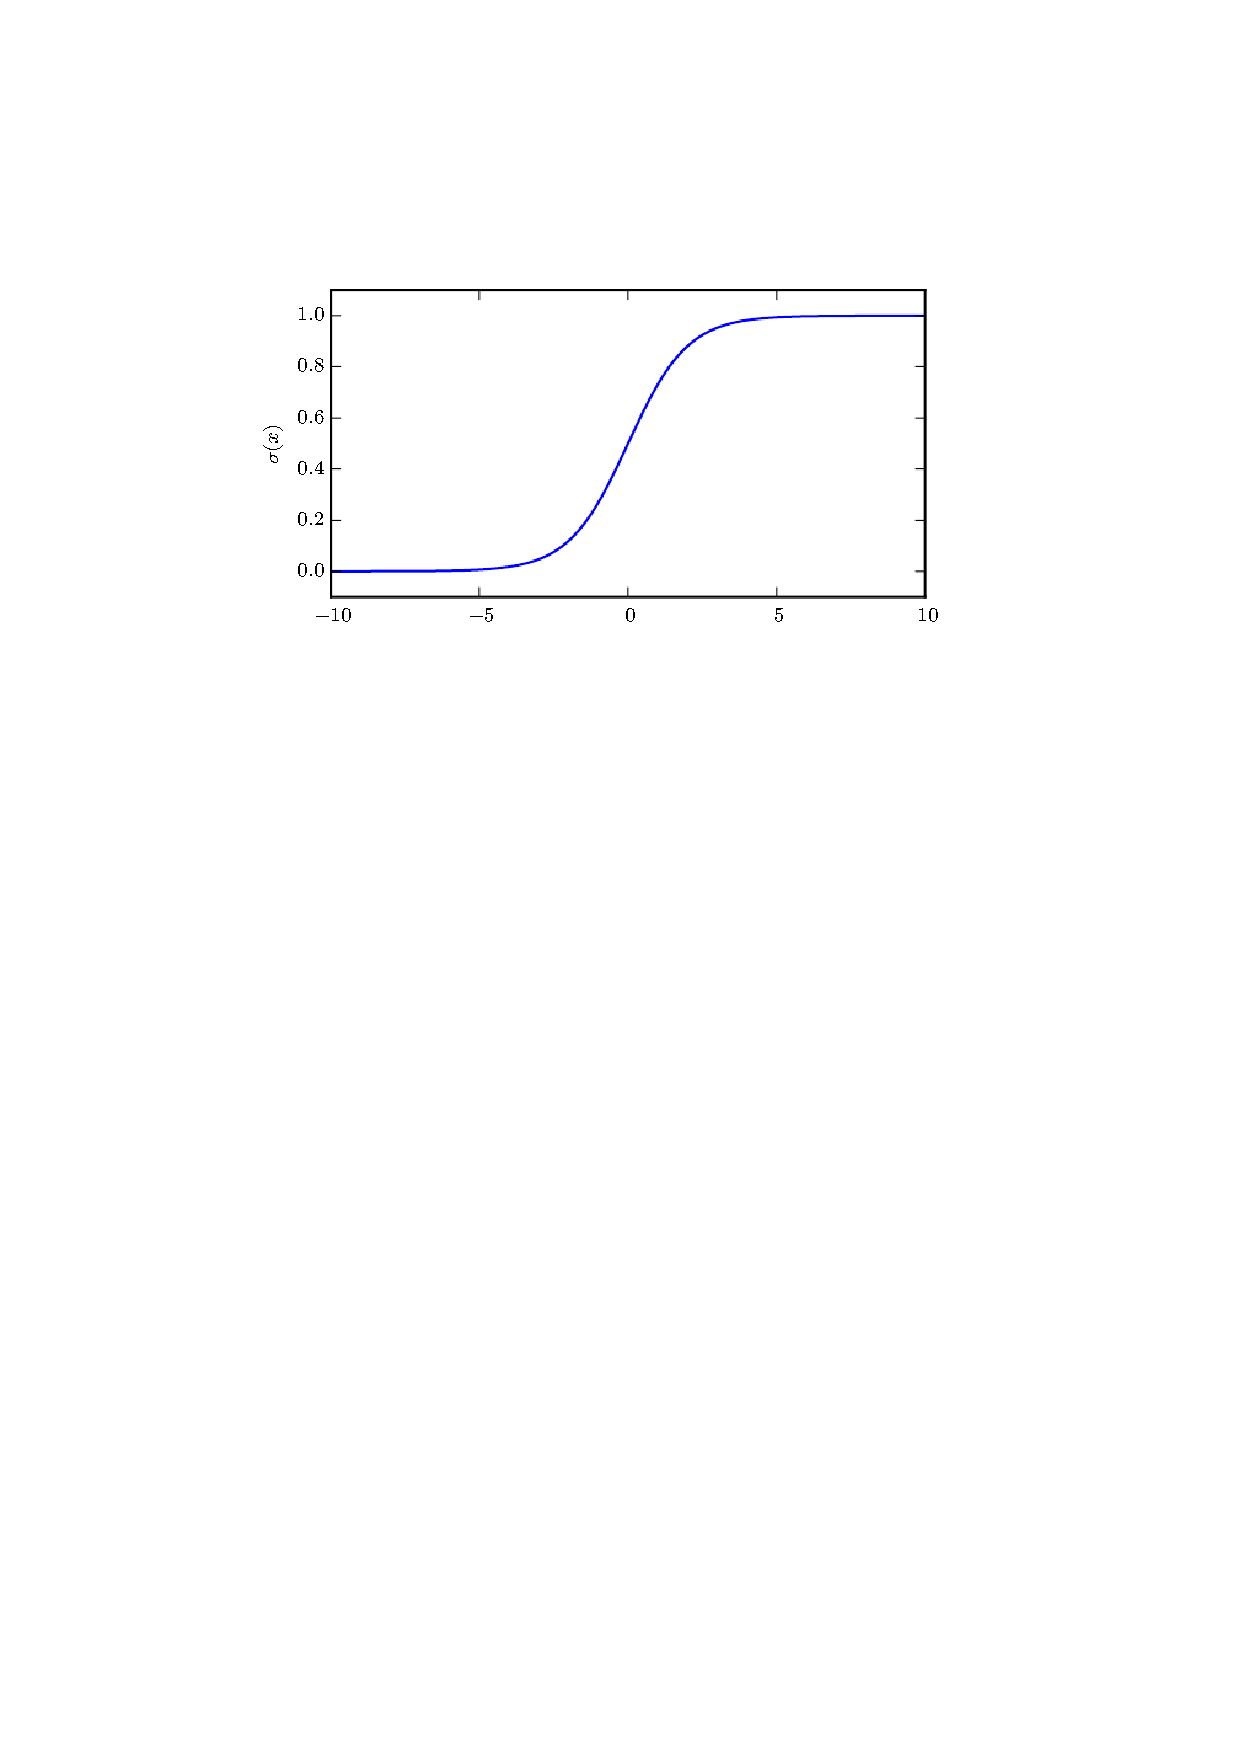
\includegraphics[width=\textwidth]{../imgs/Logistic_Sigmoid.pdf}
\end{minipage}
\paragraph{Formulas}
\begin{enumerate}
    \item $\displaystyle \sigma(x) = \frac{\exp(x)}{\exp(x) + \exp(0)}$
    \item $\displaystyle \dx{\sigma(x)} = \sigma(x) (1 - \sigma(x))$
    \item $\displaystyle 1 - \sigma(x) = \sigma(-x)$
    \item $\displaystyle \log \sigma(x) = - \zeta(-x)$
    \item $\displaystyle \sigma(x) = \dx{\zeta(x)}$
    \item $\displaystyle \forall x\in(0,1),\ \sigma^{-1}(x) = \log \left( \frac{x}{1-x} \right)$
        \begin{itemize}
            \item The function $\sigma^{-1}(x)$ is called the \textbf{logit} in statistics.
        \end{itemize}
\end{enumerate}
\paragraph{Properties}
\begin{enumerate}
    \item \textbf{Saturates} when its argument is very positive or very negative.
        \begin{itemize}
            \item very flat
            \item insensitive to small changes in its input
        \end{itemize}
\end{enumerate}
\paragraph{Applications}
\begin{enumerate}
    \item Produce the parameter of a Bernoulli distribution.
\end{enumerate}


\section{Softplus Function}
\begin{minipage}[c]{0.4\linewidth}
    \[
        \zeta(x) = \log (1 + \exp(x))
    \]
\end{minipage}
\hfill
\begin{minipage}[c]{0.6\linewidth}
    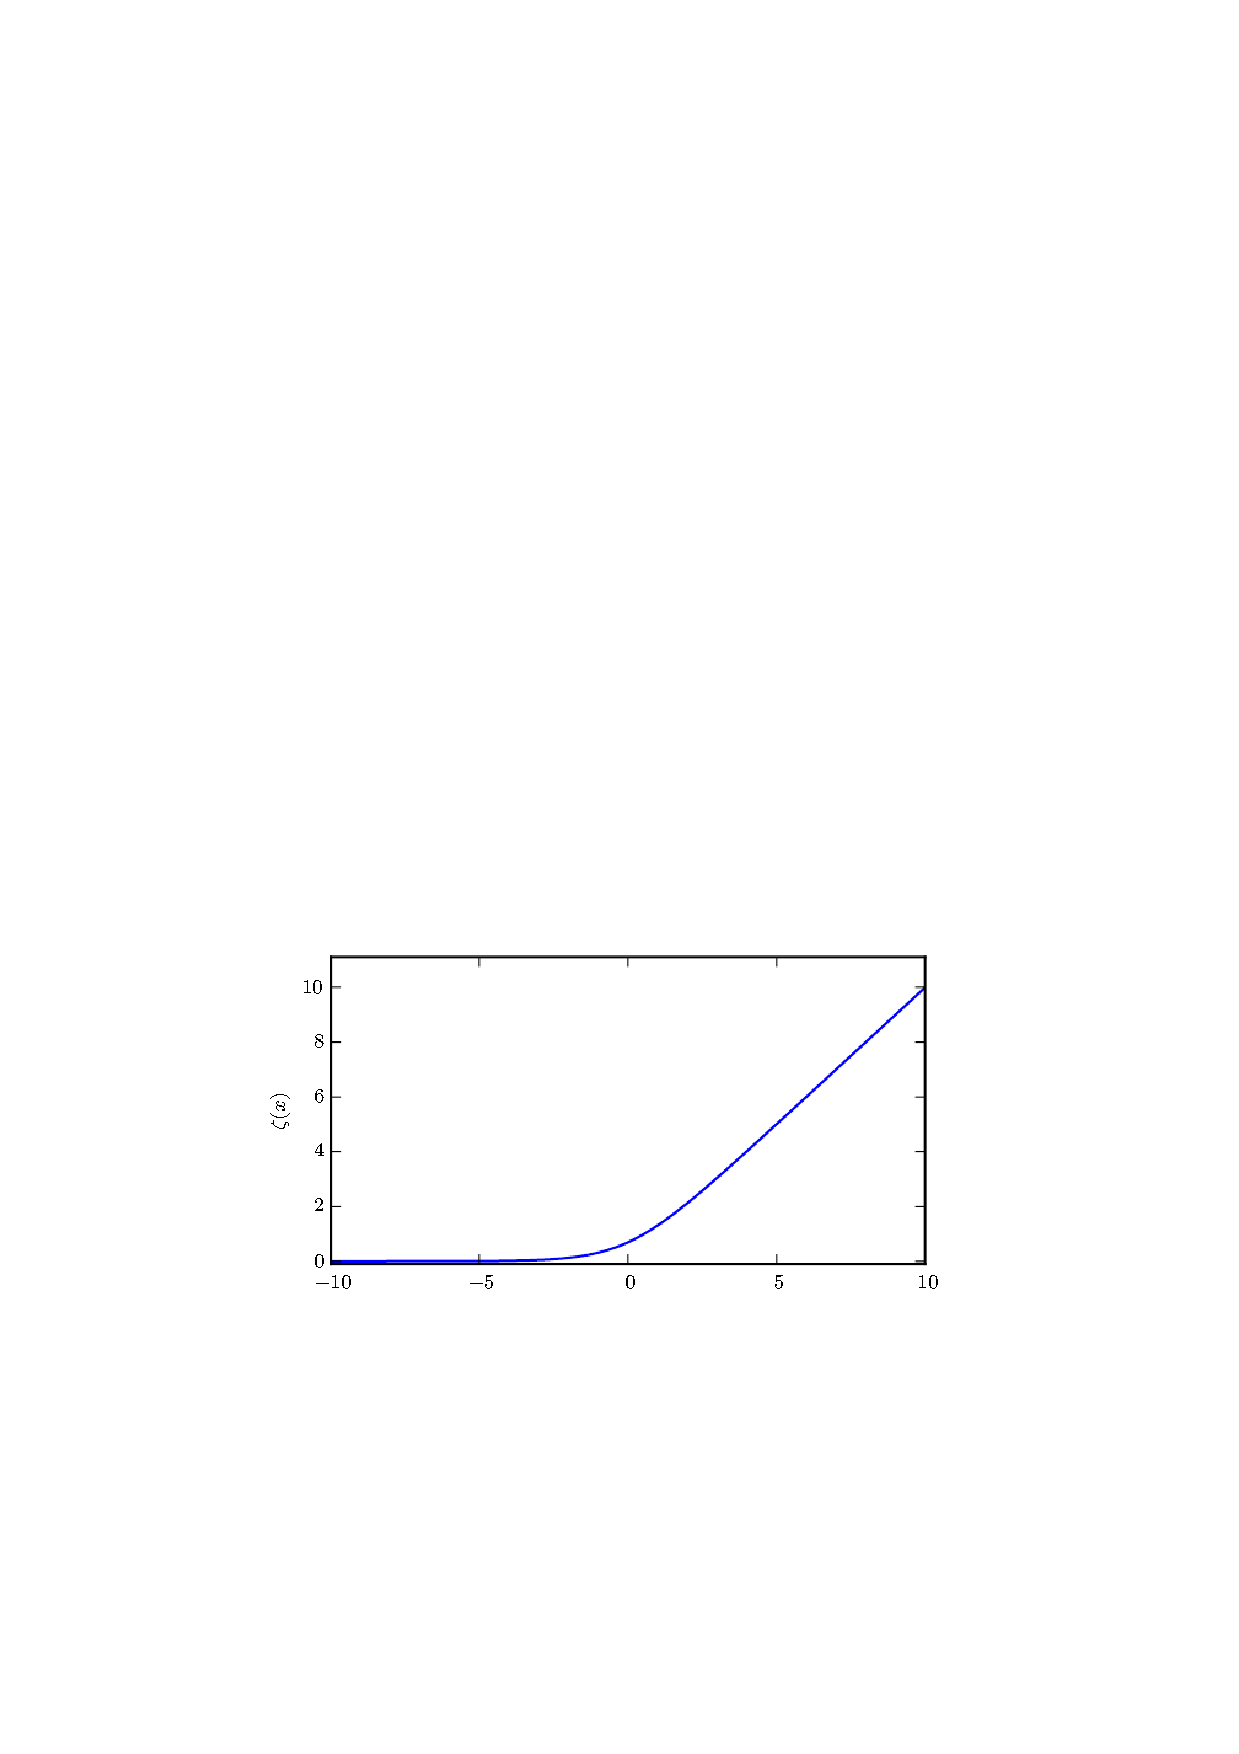
\includegraphics[width=\textwidth]{../imgs/Softplus_Function.pdf}
\end{minipage}
\paragraph{Formulas}
\begin{enumerate}
    \item $\displaystyle - \zeta(-x) = \log \sigma(x)$
    \item $\displaystyle \dx{\zeta(x)} = \sigma(x)$
    \item $\displaystyle \forall x > 0,\ \zeta^{-1}(x) = \log (\exp(x) - 1)$
    \item $\displaystyle \zeta(x) = \int_{-\infty}^x \sigma(y) \mathrm{d}y$
    \item $\displaystyle \zeta(x) - \zeta(-x) = x$
\end{enumerate}
\paragraph{Properties}
\begin{enumerate}
    \item $\zeta(x) \in (0, \infty)$
    \item $\zeta(x)$ is a smoothed (or "softened") version of
        \[
            x^+ = \max(0, x)  
        \]
        $\zeta(-x)$ is a smoothed (or "softened") version of
        \[
            x^- = \max(0, -x)  
        \]
        Similar to $x^+ - x^- = x$, we also have
        \[
            \zeta(x) - \zeta(-x) = x
        \]
\end{enumerate}
\paragraph{Applications}
\begin{enumerate}
    \item Produces the $\beta$ or $\sigma$ parameter of a normal distribution.
\end{enumerate}


\newpage
\part{Common Probability Distributions}


\section{Gaussian Distribution}
\paragraph{Introduction}
\begin{itemize}
    \item Also known as the \textbf{Normal Distribution}.
    \item The most commonly used distribution over real numbers.
\end{itemize}
\paragraph{Definition}
\subparagraph{For real numbers}
\[
    \ND{x}{\mu}{\sigma^2} = \sqrt{\frac{1}{2\pi\sigma^2}} \exp \left( -\frac{1}{2\sigma^2}(x-\mu)^2 \right)
\]
\begin{itemize}
    \item $\mu \in \mathbb{R}$
    \item $\sigma \in (0, \infty)$
\end{itemize}
\begin{center}
    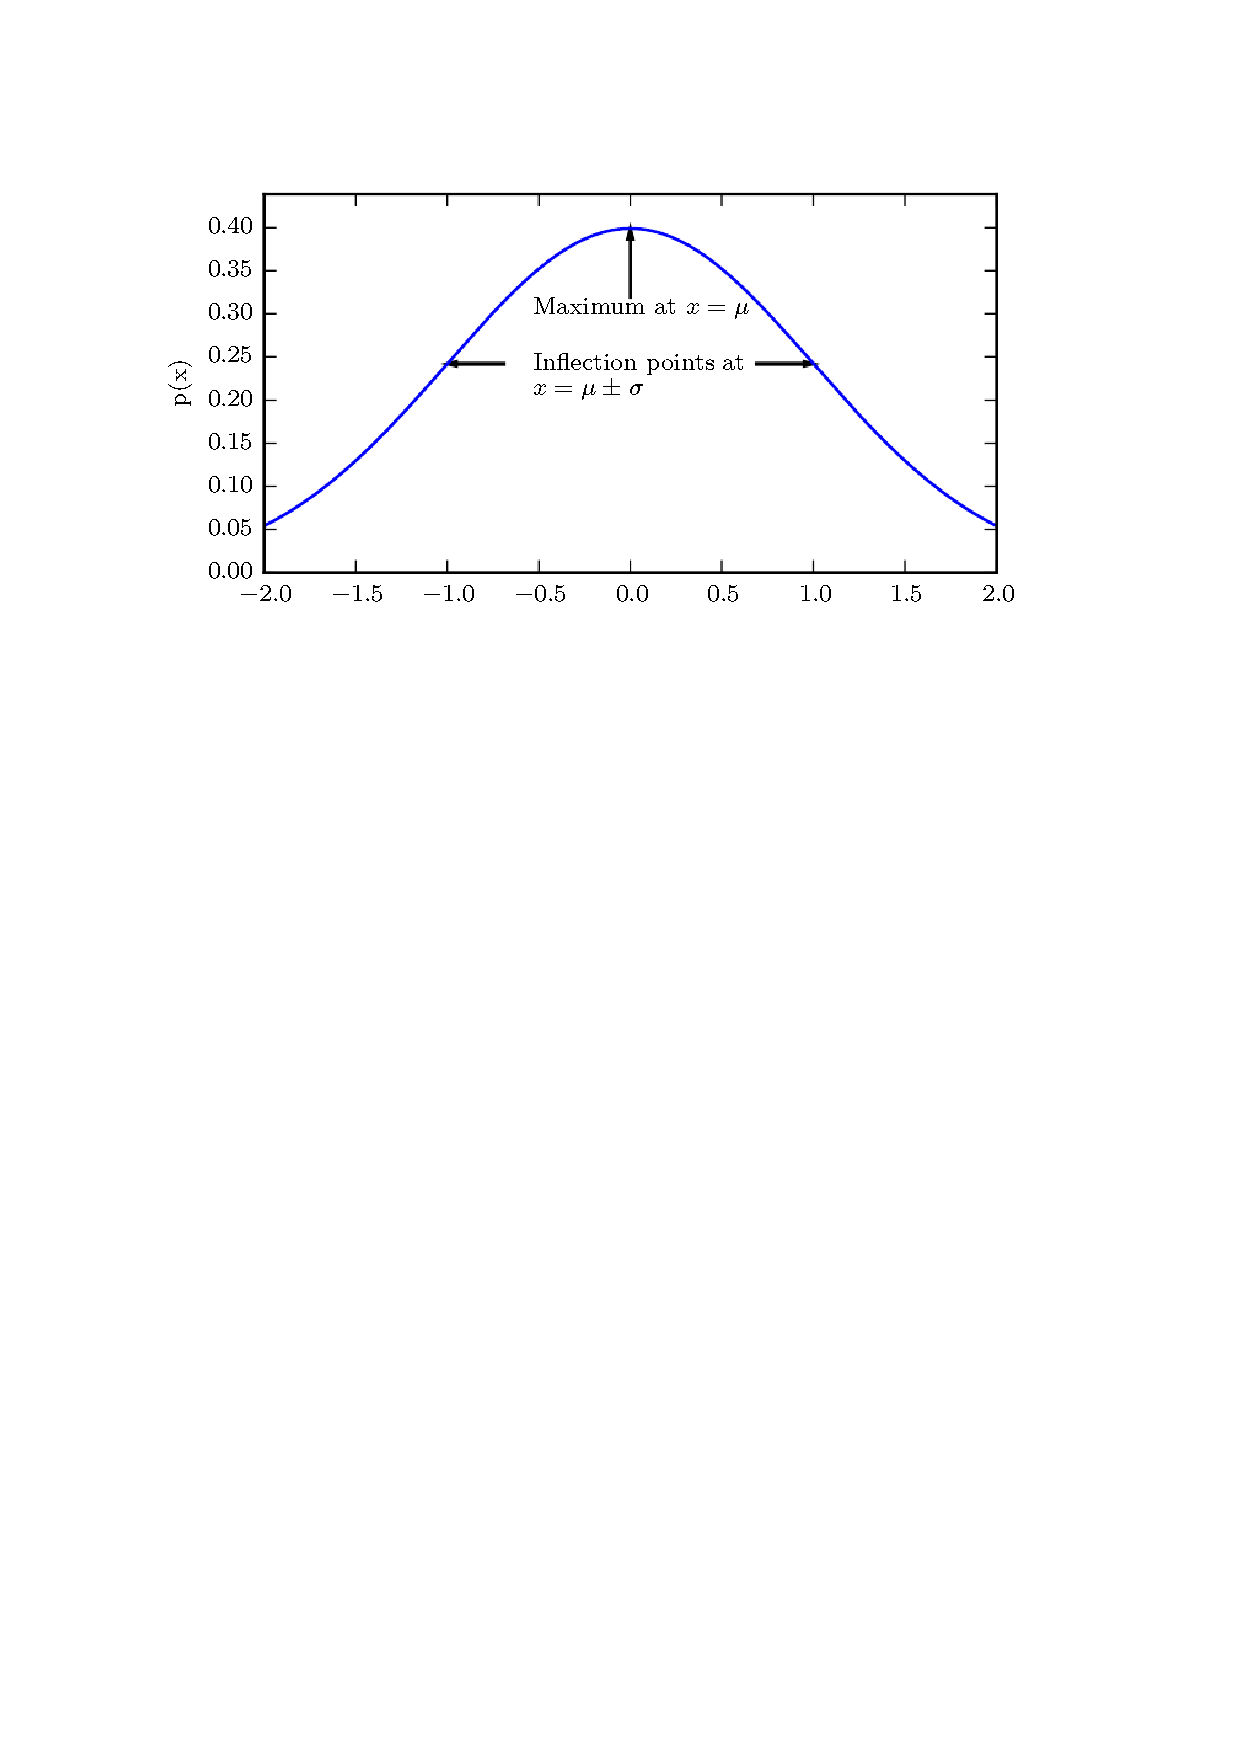
\includegraphics[width=0.8\textwidth]{../imgs/Gaussian_Distribution.pdf}    
\end{center}
\subparagraph{For $\mathbb{R}^n$}
\[
    \ND{\vx}{\vmu}{\vSigma} = \sqrt{\frac{1}{(2\pi)^n \det(\vSigma)}} \exp \left( -\frac{1}{2}(\vx-\vmu)^\top \vSigma^{-1} (\vx-\vmu) \right)
\]
\begin{itemize}
    \item Also known as \textbf{Multivariate Normal Distribution}.
    \item The covariance matrix $\vSigma$ is positive definite symmetric.
\end{itemize}
\paragraph{Variant}
\subparagraph{For real numbers}
If we need to frequently evaluate the PDF with diffrent parameter values, a more efficient way of parametrizing the distribution is to use a parameter $\beta \in (0,\infty)$ to control the \textbf{precision} (or inverse variance) of the distribution
\[
    \ND{x}{\mu}{\beta^{-1}} = \sqrt{\frac{\beta}{2\pi}} \exp\left( -\frac{1}{2}\beta(x-\mu)^2 \right)
\]
\subparagraph{For $\mathbb{R}^n$}
We can use a \textbf{precision matrix} $\vbeta$
\[
    \ND{\vx}{\vmu}{\vbeta^{-1}} = \sqrt{\frac{\det(\vbeta)}{(2\pi)^n}} \exp\left(-\frac{1}{2}(\vx-\vmu)^\top\vbeta(\vx-\vmu) \right)
\]
We often fix the covariance matrix to be a diagonal matrix. An even simpler version is the \textbf{isotropic} Gaussian distribution, whose covariance matrix is a scalar times the identiy matrix.
\paragraph{Properties}
\begin{itemize}
    \item $\mathbb{E}[x] = \mu$
\end{itemize}
\paragraph{Advantages}
\begin{enumerate}
    \item The \textbf{central limit theorem} shows that the sum of many independent random variables is approximately normally distributed.
    \item Out of all possible probability distributions with the same variance, the normal distribution encodes the maximum amount of uncertainty over the real numbers.
        \begin{itemize}
            \item We can thus think of the normal distribution as being the one that inserts the least amount of prior knowledge into a model.
        \end{itemize}
\end{enumerate}


\end{document}